\chapter{Bayesian Inference}
\label{chap:bay}
%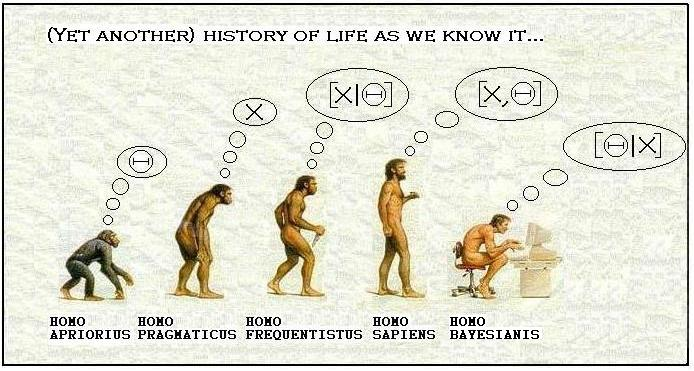
\includegraphics[width=\textwidth]{bayesian_evol}

\epigraph{We anticipate the sun will rise tomorrow, not just because it has always done so far, but because this is predicted by {\em models}, which accord with {\em data}. Any perceived failure of the sun to rise would more likely be a hallucination.}{David MacKay}


Science is not the search for truth. Instead, scientists concern themselves with the construction of models which they then determine the relative merits of using data.

% Mathematics -- if then, conditional truth
% Science -- weaker: observations -> possibilities 

\newcommand{\Probc}[2]{\mathrm{P}\left(#1\middle|#2\right)}
\newcommand{\Prob}[1]{\mathrm{P}\left(#1)}

\section{Probability}
\label{sec:bay:prob}

  We denote the probability of an event $E$, given some initial assumptions $A$ as $\Probc{E}{A}$

  \begin{figure}
    \centerline{%
      \def\firstcircle{(-0.75,0) circle (1.5)}
\def\secondcircle{(0.75,0) circle (1.5)}

\begin{tikzpicture}
  \draw \firstcircle;
  \draw \secondcircle;
  \draw (-3,-2) rectangle (3,2);

  \begin{scope}
    \fill[blue!30!white] \firstcircle;
    \clip \secondcircle;
  \end{scope}

  \begin{scope}
    \clip \firstcircle;
    \fill[blue!60!white] \secondcircle;
  \end{scope}

  \draw[above left] node at (-1,0) {\(A\)};
  \draw[above right] node at (1,0) {\(B\)};
  \draw[below ] node at (0,0) {\(A\cap B\)};
  \draw[below left] node at (3,2) {\(\Omega\)};


\end{tikzpicture}


    }
    \caption{Beer-mat mathematics. This diagram is how John Skilling explained Bayes' theorem to a young Steve Gull. Out of the entire sample space $\Omega$, if we observe $A$ to be true (blue region), then the probability of $B$ given that we know $A$ is simply $\Prob{A\cap B}/\Prob{A}$. Bayes' theorem then follows by rearrangement and symmetry.}
  \end{figure}

\section{Parameter Estimation \& Model Comparison}
\label{sec:bay:model_comp}


\section{Sampling}
\label{sec:bay:samp}

